\usetikzlibrary[positioning,fit,shadings,shapes,backgrounds,arrows,calc]

\tikzstyle{node}=[rectangle,thick,draw=black!75,fill=white!20,minimum size=6mm]

\tikzset{*|/.style={to path={(perpendicular cs: horizontal line through={(\tikztostart)},vertical line through={(\tikztotarget)}) -- (\tikztotarget) \tikztonodes}}}

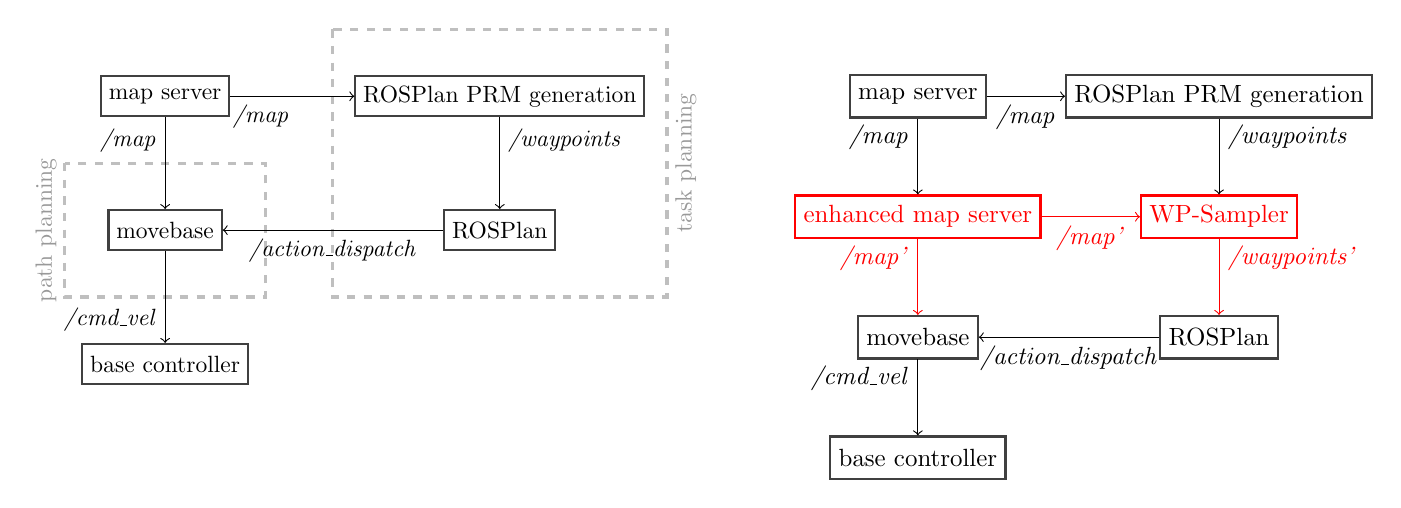
\begin{tikzpicture}[scale=0.85,every node/.style={scale=0.85}]

  \begin{scope}[local bounding box=orig](orig)
  
    \draw[black!25,very thick,dashed] (-1.5,-1) rectangle (1.5,-3);
    \draw[black!25,very thick,dashed] (2.5,1) rectangle (7.5,-3);
    
    \node at (-1.5,-2) (A) [text=black!40,anchor=south,rotate=90] {path planning};
    \node at (7.5,-1) (A) [text=black!40,anchor=north,rotate=90] {task planning};

    % nodes
    \node[node] at (0,0) (ms) {map server};
    \node[node] at (5,0) (rg) {ROSPlan PRM generation};
    \node[node] at (5,-2) (rp) {ROSPlan};
    \node[node] at (0,-2) (mb) {movebase};
    \node[node] at (0,-4) (bc) {base controller};

    \draw[->,*|] (ms.south) to node[pos=0.25,left]{\textit{/map}} (mb.north);
    \draw[->] (ms.east) to node[pos=0.25,below]{\textit{/map}} (rg.west);
    \draw[->,*|] (rg.south) to node[pos=0.25,right]{\textit{/waypoints}} (rp.north);
    \draw[->] (rp.west) to node[pos=0.5,below]{\textit{/action\_dispatch}} (mb.east);
    \draw[->,*|] (mb.south) to node[pos=0.75,left]{\textit{/cmd\_vel}} (bc.north);

  \end{scope}

  \begin{scope}[xshift=32em,scale=0.9,every node/.style={scale=0.9}](new)
  
    % \draw[black!25,very thick,dashed] (-1.5,-3) rectangle (1.5,-5);
    % \draw[black!25,very thick,dashed] (2.5,1) rectangle (7.5,-5);
    
    % \node at (-1.5,-4) (A) [text=black!40,anchor=south,rotate=90] {path planning};
    % \node at (7.5,-1) (A) [text=black!40,anchor=north,rotate=90] {task planning};

    % nodes
    \node[node] at (0,0) (ms) {map server};
    \node[node] at (5,0) (rg) {ROSPlan PRM generation};
    \node[node] at (5,-2) (ws) [draw=red,text=red] {WP-Sampler};
    \node[node] at (5,-4) (rp) {ROSPlan};
    \node[node] at (0,-2) (sm) [draw=red,text=red] {enhanced map server};
    \node[node] at (0,-4) (mb) {movebase};
    \node[node] at (0,-6) (bc) {base controller};

    \draw[->,*|] (ms.south) to node[pos=0.25,left]{\textit{/map}} (sm.north);
    \draw[->,*|,draw=red] (sm.south) to node[pos=0.25,left,text=red]{\textit{/map'}} (mb.north);
    \draw[->] (ms.east) to node[pos=0.5,below]{\textit{/map}} (rg.west);
    \draw[->,*|] (rg.south) to node[pos=0.25,right]{\textit{/waypoints}} (ws.north);
    \draw[->,draw=red] (sm.east) to node[pos=0.5,below,text=red]{\textit{/map'}} (ws.west);
    \draw[->,*|,draw=red] (ws.south) to node[pos=0.25,right,text=red]{\textit{/waypoints'}} (rp.north);
    \draw[->] (rp.west) to node[pos=0.5,below]{\textit{/action\_dispatch}} (mb.east);
    \draw[->,*|] (mb.south) to node[pos=0.25,left]{\textit{/cmd\_vel}} (bc.north);
    
  \end{scope}

\end{tikzpicture}